\chapter{O Câncer no Mundo}
\label{chapter:o_cancer_no_mundo}

Denominado, também, como neoplasia ou tumor maligno, o câncer é um conjunto de
mais de 100 doenças, em que há um crescimento exacerbado de células em um
determinado tecido. Essas células, por sua vez, podem se espalhar a tal ponto,
que chegam a atingir outros órgãos e tecidos, fenômeno denominado de
“metástase”, demonstrando o poder agressivo dessa classe de patologias.\cite{OQUEECANCER}

Para o ano de $2018$ era estimado uma incidência de $18,1$ milhões de novos casos de câncer no mundo.
Também foi datado, no mesmo ano, $9,6$ milhões de óbitos \cite{MOC}, como mostrado na figura \ref{fig:cancerdata}.

\begin{figure}[H]
\begin{center}
\caption{Incidência mundial de câncer}
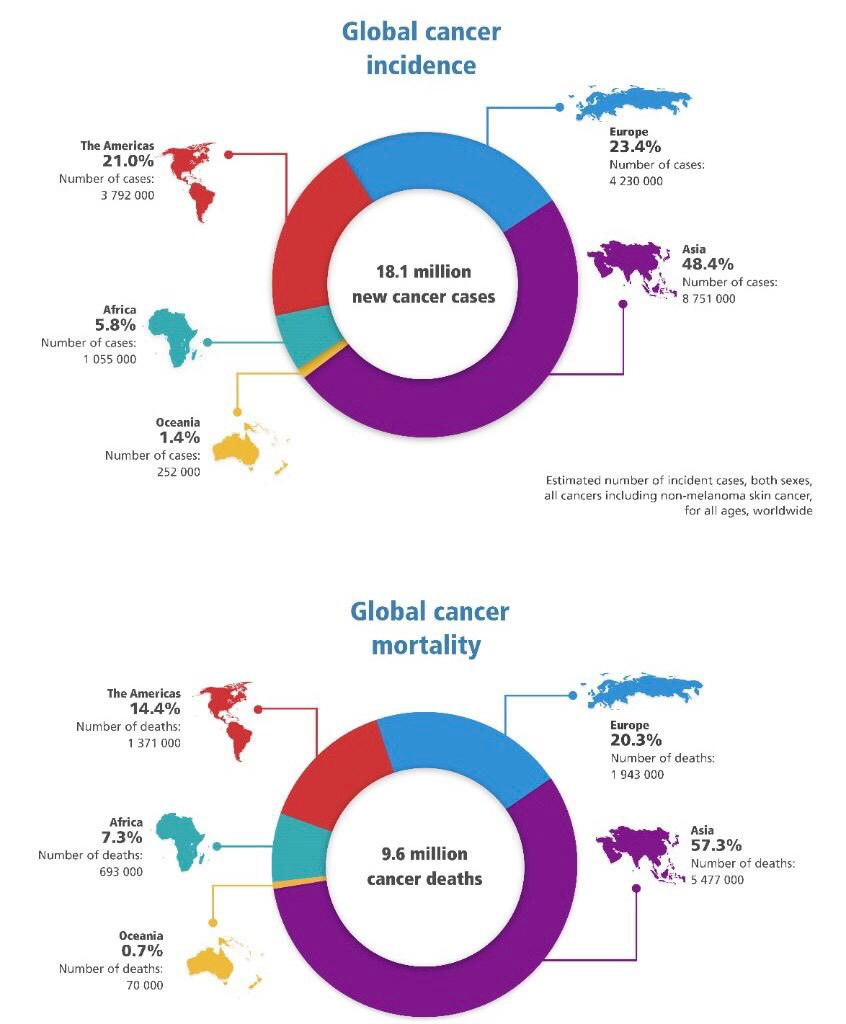
\includegraphics[width=12cm]{cancerdata}
\label{fig:cancerdata}
\end{center}
\legend{Fonte: \url{https://www.iarc.fr/wp-content/uploads/2018/09/Globocan\_01.jpg} \cite{GLOBOCAN} }
\end{figure}

\section{\textbf{Etapas do diagnóstico de câncer}}

O diagnóstico tem como definição ser o processo de identificação a partir de
exames médicos, sintomas e sinais além das amostras do tecido atingido.\cite{ATLAS}

Assim, até que o Patologista, especialista médico responsável pelo laudo anatomopatológico,
faça sua resolução, há alguns processos que auxiliam na análise do problema.
Dentre os exames mais solicitados, está a retirada de um fragmento do tecido suspeito,
para que possa ser feita uma análise em laboratório no microscópio afim de verificar aspecto dos núcleos e
a morfologia das células presentes naquela amostra;
exames de sangue, da medula óssea; radiografia; ultrassonografia, ressonância magnética;
tomografia computadorizada por emissão de pósitrons (PET-TC), são exemplos de exames convencionais.\cite{VENCER}

É importante destacar que a solicitação desses procedimentos irá variar de acordo com a suspeita do tumor,
além da necessidade de uma avaliação mais abrangente,
pois há situações em que os exames convencionais não expõem a informação necessária para um diagnóstico definitivo.
E em alguns casos é preciso a realização de exames Imunohistoquímicos (IHQ), com marcações especiais.

Todo esse processo é de extrema importância, pois, apenas a partir da análise desses laudos,
pelo médico responsável, que ele poderá, confirmar ou descartar a hipótese da neoplasia, e em caso de confirmação,
iniciar um plano de tratamento específico para o problema.


\section{\textbf{Importância do diagnóstico precoce}}

O processo de identificação, exame e avaliação do câncer requer vários fatores, e, portanto, requer tempo.

Porém, profissionais e órgãos da área de saúde alertam para a importância de um diagnóstico precoce,
pois esse, pode elevar as chances de um prognóstico favorável ao paciente.

O Ministério da Saúde do Brasil relata a importância de um diagnóstico em estágios iniciais da seguinte maneira:

“O objetivo do diagnóstico precoce é identificar pessoas com sinais e sintomas iniciais da doença,
primando pela qualidade e pela garantia da assistência em todas as etapas da linha de cuidado da doença.
O diagnóstico precoce, portanto, é uma estratégia que possibilita terapias mais simples e efetivas,
ao contribuir para a redução do estágio de apresentação do câncer.
Assim, é importante que a população em geral e os profissionais de saúde reconheçam os sinais de alerta dos cânceres mais comuns,
passíveis de melhor prognóstico se descobertos no início.
A maioria dos cânceres é passível de diagnóstico precoce mediante avaliação e encaminhamento após os primeiros sinais e sintomas.”
\cite{DIAGNOSTICO}

